In this section we discuss the method of linear regression. Here, we consider the following setting.

\begin{itemize}
    \item We begin with a collection of data $D_n := \{(a_1, y_1), \ldots, (x_n, y_n)\}$
    \item We assume the data has the form (assume a model i.e. linear regression) $y = X\beta + \varepsilon$
    \item Input space $\mathcal{X} = \mathbb{R}^p$; Outcome space $\mathcal{Y} = \mathbb{R}$.
    \item Action spcae (sometimes called \textit{hypothesis space}) $\mathcal{A}^{\mathcal{X}} := \{f_w \vert w \in \mathbb{R}^p\}$ where
    $$f_w : x \mapsto w^\top x. $$
\end{itemize}

In this case,

$$X = 
\begin{bmatrix}
  --- &  x_1^\top & ---  \\
  --- &  x_2^\top & --- \\
  --- &  \vdots & --- \\
  --- &  x_n^\top & ---
\end{bmatrix}, \text{  }
y = 
\begin{bmatrix}
y_1 \\ y_2 \\ \vdots \\ y_n    
\end{bmatrix}$$

\vspace{0.2cm}

\begin{remark}
    Some important facts to consider:
    \begin{enumerate}
        \item Sometimes, we want to do some data pre-processing. This means we might want to center our data i.e. $x_i^c = x_i - \bar{x}$ and we might
    also want to normalize.
        \item Note that $X \in \mathbb{R}^{n \times p}$; the \textit{design matrix} whose $i^{\text{th}}$ row is $x_i^\top$.
    \end{enumerate}
\end{remark}

It is important to note that linear regression is basically us assuming that our data takes the shape of our model (i.e. $y = X\beta + \varepsilon$) where
we also need an \textit{estimator} $\hat{\beta}$ i.e. a `way' to aproximate $\beta$. In the previous section, we explored such a method to do this; recall Ordinary Least Squares (OLS).

\begin{remark}
The \emph{risk} of a predictor $f_w(x) = w^\top x$ under squared loss is
\[
R(w) = \mathbb{E}\big[(Y - w^\top X)^2\big],
\]
where the expectation is taken with respect to the (unknown) distribution of $(X,Y)$.
Since this expectation cannot be computed directly, we approximate it by the
\emph{empirical risk}:
\[
\hat R_n(w) = \frac{1}{n}\sum_{i=1}^n (y_i - w^\top x_i)^2.
\]
This corresponds to replacing the population expectation with the sample average.
By the law of large numbers, $\hat R_n(w) \to R(w)$ as $n \to \infty$.
Thus, empirical risk minimization provides a practical way to approximate
population risk.
\end{remark}

When we consider this in a vectorized form, we obtain that
$$\hat R_n(w) = \frac{1}{n}\sum_{i=1}^n (y_i - w^\top x_i)^2 = \frac{1}{n} \vert \vert {y - Xw}\vert \vert_2^2$$

In order to minimize this risk, i.e. solve $\text{min}_{w \in \mathbb{R}^d} \hat{\mathcal{R}}(\hat{f_w})$ we consider that 
$$\hat R_n(w) = \frac{1}{n} \left( w^\top X^\top X w - 2 w^\top X^\top y + \vert \vert y \vert \vert_2^2 \right)$$
is a \textit{differentiable convex} function, whose minima are then characterized by the equation $$X^\top X w - X^\top y = 0.$$

Thus, if $X^\top X$ is invertible, the equation above has a unique solution (the one we found in the previous section! \ref{sec:ex01}) and thus, our \textit{empirical risk minimizer} $\hat f$ is given by 
$$\hat f : x \prime \mapsto x\prime^\top\left(X^\top X\right)^{-1}X^\top y$$

\begin{definition}
A function $f : \mathbb{R}^d \to \mathbb{R}$ is said to be \emph{differentiably convex}
if it is both differentiable and convex.

\begin{itemize}
  \item \textbf{Differentiable:} $f$ is differentiable at $x\in\mathbb{R}^d$ if the gradient
  $\nabla f(x)$ exists, i.e.\ there is a linear map $g:\mathbb{R}^d\to\mathbb{R}$ such that
  \[
  \lim_{h\to 0}\frac{f(x+h)-f(x)-g(h)}{\|h\|}=0.
  \]

  \item \textbf{Convex:} $f$ is convex if for all $x,y\in\mathbb{R}^d$ and $t\in[0,1]$,
  \[
  f(tx+(1-t)y)\leq t f(x)+(1-t)f(y).
  \]
  Equivalently, if $f$ is differentiable, convexity is equivalent to the first-order condition
  \[
  f(y)\geq f(x) + \nabla f(x)^\top (y-x)\quad \forall x,y\in\mathbb{R}^d.
  \]

  \item \textbf{Strict convexity:} $f$ is strictly convex if for all $x\neq y$ and $t\in(0,1)$,
  \[
  f(tx+(1-t)y) < t f(x)+(1-t)f(y).
  \]
  In the differentiable case, this implies that the first-order inequality is strict whenever $y\neq x$.
\end{itemize}

Thus, a differentiably convex function is one that admits a gradient and satisfies the convexity inequalities.
\end{definition}

\textbf{slight problemo amigo:} Whenever $p > n$, $X^\top X$ is not invertible, this gives our equation multiple solutions (not unique anymore).

\subsection*{Linear regression v. Affine regression}
$$f_w (x) = w^\top x \text{     v.     } f_{w, b} (x) = w^\top x + b = \hat{w}^\top \hat{x}$$
where
$$\hat{w} = \begin{bmatrix}
    w \\ b
\end{bmatrix}, \text{   } \hat{x} = \begin{bmatrix}
    x \\ 1
\end{bmatrix}$$

\begin{remark}
    Wowoweeewa, this shows that an affine regression of dimention $p$ is just a linear regresion of dimention $p + 1$! Then, these two models are equivalent if we do not \textit{regularize}
    (this is true because $b$ is usually not regularized).
\end{remark}

\subsection*{Hat matrix and porn (geometry of linear regression)}
If $X\in\mathbb{R}^{n\times p}$ has full column rank, then the OLS estimator is
\[
\hat w = (X^\top X)^{-1}X^\top y,
\]
so that for the training data we obtain
\[
\hat y = X\hat w = X(X^\top X)^{-1}X^\top y = Hy,
\]
with
\[
H = X(X^\top X)^{-1}X^\top.
\]

\medskip

\noindent
Let $r = \operatorname{rank}(X)$. Consider the eigenvalue decomposition of $XX^\top$ in reduced form:
\[
XX^\top = USU^\top,
\]
where
\begin{itemize}
  \item $U \in \mathbb{R}^{n\times r}$ is an orthonormal matrix (its columns form an orthonormal basis for $\operatorname{Im}(X)$),
  \item $S \in \mathbb{R}^{r\times r}$ is a diagonal matrix with strictly positive entries.
\end{itemize}
Then one can show that
\[
H = UU^\top.
\]

\medskip

\noindent
\textbf{Geometric interpretation:} The hat matrix $H$ (called hat matrix cuz' it maps $y$ to $\hat y$ hence adding a hat to it) is the orthogonal projector onto $\operatorname{Im}(X)$.
The geometry produced by this projection may be observed in the following figure \ref{fig:linreg_geometry}

\vspace{0.2cm}

This means:
\begin{itemize}
  \item The fitted vector $\hat y = Hy$ is the projection of $y$ onto the subspace $\operatorname{Im}(X)$ (the span of the columns of $X$).
  \item The residual vector $y - \hat y$ lies in $\operatorname{Im}(X)^\perp$.
\end{itemize}

\medskip

\noindent
In the case $X = [x^{(1)} \; x^{(2)}] \in \mathbb{R}^{n\times 2}$, the column space $\operatorname{Im}(X)$ is the plane spanned by $x^{(1)}$ and $x^{(2)}$. The observed vector $y$ is projected onto this plane, producing $\hat y = Hy$, and the residual $y - \hat y$ is orthogonal to it.

\begin{figure}[htbp]
\centerline{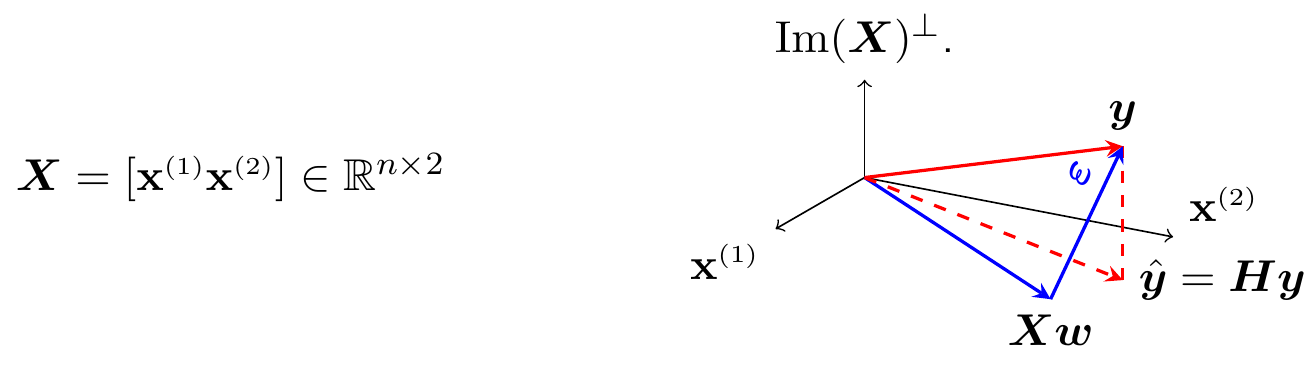
\includegraphics[scale=.2]{figures/geometry_linearRegression.png}}
\caption{Geometry of linear regression}
\label{fig:linreg_geometry}
\end{figure}

\subsection*{Optimality of least squares linear regression}
Assuming that $y = X\beta + \varepsilon$ where $\operatorname{rank}(X) = p$ i.e. full rank matrix and \textit{decorrelated centered noise} $\mathbb{E}[\varepsilon] = 0; \text{  } \mathbb{E}[\varepsilon^\top \varepsilon] = \sigma^2I$.

\begin{theorem}
    Gauss-Markov Theorem: Assuming the previous statements, $\hat \beta = \left( X^\top X\right)^{-1} X^\top y$ is the \textit{best linear unbiased estimator} (BLUE). That is, for any other \textit{unbiased} estimator $\tilde{\beta}$ we have
    $$\operatorname{Cov}(\tilde \beta) = \operatorname{Cov} (\hat \beta) + K_{\tilde \beta}$$ where $K_{\tilde \beta}$ is a \textit{possitive semi-definite} matrix. 
\end{theorem}

\begin{remark}[Positive (semi)definiteness]
A symmetric matrix $M \in \mathbb{R}^{d\times d}$ is called
\begin{itemize}
  \item \emph{positive semidefinite (psd)} if
  \[
  z^\top M z \;\geq\; 0 \quad \forall z \in \mathbb{R}^d,
  \]
  written $M \succeq 0$.
  \item \emph{positive definite (pd)} if
  \[
  z^\top M z \;>\; 0 \quad \forall z \in \mathbb{R}^d\setminus\{0\},
  \]
  written $M \succ 0$.
\end{itemize}
Equivalently:
\begin{itemize}
  \item $M\succeq 0$ if and only if all eigenvalues of $M$ are nonnegative,
  \item $M\succ 0$ if and only if all eigenvalues of $M$ are strictly positive.
\end{itemize}
\end{remark}

\subsection*{Gaussian conditional model and least squares regression}

We can model the conditional distribution of $Y$ given $X$ as
\[
Y \mid X \sim \mathcal{N}(\beta^\top X, \sigma^2).
\]

\begin{itemize}
  \item Likelihood for one observation $(x_i,y_i)$:
  \[
  p(y_i \mid x_i) = \frac{1}{\sqrt{2\pi\sigma^2}}
  \exp\!\left(-\frac{1}{2\sigma^2}(y_i - \beta^\top x_i)^2\right).
  \]

  \item Negative log-likelihood:
  \[
  -\ell(\beta,\sigma^2) = 
  \sum_{i=1}^n -\log p(y_i\mid x_i)
  = \frac{n}{2}\log(2\pi\sigma^2) 
  + \frac{1}{2\sigma^2}\sum_{i=1}^n (y_i - \beta^\top x_i)^2.
  \]
\end{itemize}

\medskip

\noindent Minimization over both $\beta$ and $\sigma^2$ yields:
\[
\min_{\sigma^2,\beta} \; 
\frac{n}{2}\log(2\pi\sigma^2) 
+ \frac{1}{2\sigma^2}\|y - X\beta\|_2^2.
\]

\begin{remark}
For fixed $\sigma^2$, minimizing in $\beta$ is equivalent to the
usual least squares problem:
\[
\min_{\beta} \; \frac{1}{2\sigma^2}\|y - X\beta\|_2^2.
\]
Optimizing over $\sigma^2$ gives the maximum-likelihood estimate:
\[
\hat\sigma^2_{\mathrm{MLE}} = \frac{1}{n}\sum_{i=1}^n (y_i - \hat\beta^\top_{\mathrm{MLE}} x_i)^2.
\]
\end{remark}

\subsection*{Properties if the model is well-specified}

Assume
\[
y = X\beta^\ast + \varepsilon,
\]
with full column rank design matrix ($\operatorname{rank}(X)=p$,
thus $n \geq p$) and i.i.d.\ centered Gaussian noise
$\varepsilon \sim \mathcal{N}(0,\sigma^2 I)$.

\begin{proposition}[Distributional properties]
  Under these assumptions:
  \begin{itemize}
  \item $\hat\beta = (X^\top X)^{-1}X^\top y 
  \;\sim\; \mathcal{N}\!\big(\beta^\ast,\, \sigma^2 (X^\top X)^{-1}\big)$
  \item $S^2 = \frac{1}{n-p}\,\|y - \hat y\|_2^2 
  \;\sim\; \sigma^2 \cdot \frac{1}{n-p}\chi^2_{n-p}$
  \item $\hat\beta \;\perp\!\!\!\perp\; S^2$
  \end{itemize}
\end{proposition}

\begin{remark}
These distributional facts are the foundation for classical inference tools:
ANOVA, $t$-tests, and confidence intervals. They are only valid
if the Gaussian linear model is correctly specified
(i.e.\ the noise is truly Gaussian and homoscedastic).
\end{remark}